% --------------------------------------------------------------
% This is all preamble stuff that you don't have to worry about.
% Head down to where it says "Start here"
% --------------------------------------------------------------
 
\documentclass[12pt]{article}
 
\usepackage[nouppercase,headsepline,footsepline,plainfootsepline]{scrpage2}
\automark{section}
\pagestyle{scrheadings}
%\clearscrheadfoot
\ihead{Math 521\;\; Oct 26, 2018}
%\ofoot[\pagemark]{\pagemark}% Optional argument controls chapter-starting pages
\ifoot[(Author)]{{\sl \hfill Meenmo K.}}

\usepackage[margin=1in]{geometry} 
\usepackage{amsmath,amsthm,amssymb,scrextend}
\usepackage{fancyhdr}
\usepackage{enumitem}
\usepackage{amsmath}
\usepackage{amssymb}
\usepackage{textcomp}
\usepackage{fancybox}
\usepackage{tikz}
\usepackage{cancel}
\usepackage{tasks}


\newcommand{\N}{\mathbb{N}}
\newcommand{\Z}{\mathbb{Z}}
\newcommand{\I}{\mathbb{I}}
\newcommand{\R}{\mathbb{R}}
\newcommand{\Q}{\mathbb{Q}}
\renewcommand{\qed}{\hfill$\blacksquare$}
\let\newproof\proof
\renewenvironment{proof}{\begin{addmargin}[1em]{0em}\begin{newproof}}{\end{newproof}\end{addmargin}\qed}
% \newcommand{\expl}[1]{\text{\hfill[#1]}$}
\setlength{\parindent}{0pt}
\newenvironment{theorem}[2][Theorem]{\begin{trivlist}
\item[\hskip \labelsep {\bfseries #1}\hskip \labelsep {\bfseries #2.}]}{\end{trivlist}}
\newenvironment{lemma}[2][Lemma]{\begin{trivlist}
\item[\hskip \labelsep {\bfseries #1}\hskip \labelsep {\bfseries #2.}]}{\end{trivlist}}
\newenvironment{problem}[2][Problem]{\begin{trivlist}
\item[\hskip \labelsep {\bfseries #1}\hskip \labelsep {\bfseries #2.}]}{\end{trivlist}}
\newenvironment{exercise}[2][Exercise]{\begin{trivlist}
\item[\hskip \labelsep {\bfseries #1}\hskip \labelsep {\bfseries #2.}]}{\end{trivlist}}
\newenvironment{reflection}[2][Reflection]{\begin{trivlist}
\item[\hskip \labelsep {\bfseries #1}\hskip \labelsep {\bfseries #2.}]}{\end{trivlist}}
\newenvironment{proposition}[2][Proposition]{\begin{trivlist}
\item[\hskip \labelsep {\bfseries #1}\hskip \labelsep {\bfseries #2.}]}{\end{trivlist}}
\newenvironment{corollary}[2][Corollary]{\begin{trivlist}
\item[\hskip \labelsep {\bfseries #1}\hskip \labelsep {\bfseries #2.}]}{\end{trivlist}}
 
 
\begin{document}

\begin{block}{\bf Theorem} Let $f:[a,b] \rightarrow \mathbb{R}$ be continuous, $f(a)<(b)$. Then $\forall\;v\in (f(a),f(b)),\;\exists\;c\in (a,b)$ such that (f(c)=v). [image1]
\end{block}

{\sl Proof.}
\begin{itemize}
    \item We inductively define a sequence of intervals $[a_n,b_n]$ and $f(a_n)<v<f(b_n)\;\forall n$.
    \item Let $[a_0,b_0]=[a,b]$, let $c_0 = \frac{a+b}{2}$.
    \item If $f(c_0) <v,$ let $[a_1,b_1] = [c_0, b_0]$.
    \item If $f(c_0)>v,$ let $[a_1,b_1]=[a_0,c_0]$.
    \item So $f(a_1)<v<f(b_1)$, $|b_1-a_1| = \frac{1}{2}|b-a|$.
    \item Inductively, suppose we have $[a_0,b_0],...,[a_n,b_n]$.
    \item Let $c_n = \frac{a_n+b_n]}{2}$.
    \item If $F(c_n)<v$, let $[a_{n+1},b_{n+1}] = [c_n,b_n]$.
    \item If $F(c_n)>v$, let $[a_{n+1},b_{n+1}] = [c_n,c_n]$.
    Note if $f(c_n)=v$, we are done.
    \item Then $\forall n, |b_n-a_n| \le \frac{1}{2^n} |b-a|, [a_n,b_n]\supset [a_{n+1},b_{n+1}], f(a_N)<v<f(b_n)$.
    \item As $(a_n)$ is monotone and bounded by $a\lea_n\leb, a_n \longrightarrow c\in[a,b].$
    \item Also, $b_n$ is monotone and bounded, so $b_n\longrightarrow c' \in [a,b]$.
    \item As $f$ is continuous, $f(c) = \lim f(a_n)\le v, f(c) = \lim f(b_n) \ge v$.
    \item So $f(c) = v$.
\end{itemize}

\vspace{1.5\baselinestretch}
\begin{block}{\bf Example} Existence of square root.\\
Let $a>0$, then $\exists\;x>0$ such that $x^2=a$.
\begin{itemize}
    \item Let $f:[0,\infty)\rightarrow\mathbb{R}$ be $f(x) = x^2$.
    \item Note f is continuous and $f(0)=0<a, f(a+1) = (a+1)^2 > a+1>a$.
    \item So by IVT, $\exists\;x\in(0,a+1)$ such that $f(x)=a,$ i.e.$x^2=a$.
\end{itemize}
\end{block}

\begin{block}{\bf Theorem} Continuous Inverse Function Theorem\\
Let $f:[a,b]\rightarrow\mathbb{R}$ be continuous and strictly increasing. Then $f^{-1}:[f(a),f(b)]\rightarrow [a,b]$ is well-defined and continuous.\end{block}

\vspace{1.5\baselinestretch}
{\sl Proof.}
\begin{itemize}
    \item As $f$ is strictly increasing, it is injective.
    \item Let $v\in (f(n), f(b)),$ then as $f(a)<f(b), \exists\;c\in(a,b)$ such that $f(c)=V$ by IVT.
    \item Hence $f$ is bijective, so $f^{-1}$ well-0defined.
    \item To show continuity, let $\mathbb{O}\subset[a,b]$ be open.
    \item Show $(f^{-1})^{-1}(O)$ is open.
    \item As $f, f^{-1}$ are bijective, $(f^{-1})^{-1}(\O) = f(O).$
    \item as $O$ is open, $O^c$ is closed, $O^c \subset[a,b],$ hence $O^c$ is compact.
    \item By theorem 4.10, as $f$ is continuous, $fO^c)$ is also compact, hence closed.
    \item So $f(O)^c = f(O^c)$ is closed, so $f(O)$ is open.
\end{itemize}

\vspace{1.5\baselineskip}
\begin{block}{\bf Theorem}
Let X,Y be metric spaces X compact, $f: X\rightarrow Y$ a continuous bijection. Then $f^{-1}$ exists and is continuous.
\end{block}

\vspace{1.5\baselineskip}
{\bf 4.4 Uniform Continuity}\\

\begin{block}{\bf Definition} Let X<Y be metric spaces, $f: X\rightarrow Y$. We say $f$ is {\sl uniformly continuous} if $\forall\;\epsilon>0$ such that $\forall\;p,q\inX$ with $d(p,q)<\delta$, we have $d(f(p),f(q))<\epsilon.$\\
{\sl Note. $\delta$ depends only on $\epsilon$, not on $p,q$.}

\vspace{1.5\baselineskip}
\begin{block}{\bf Theorem} Let $f: X\rightarrow Y$. Then $f$ is uniformly continuous if and only if for any parir of sequences $(p_n), (q_n) \subset X$ such that $d(p_n, q_n)\rightarrow 0, d(f(p_n),f(q_n))\rightarrow 0$.\\
{\sl Note. $p_n,q_n$ do not have to converge. e.g. $p_n = n, q_n = n+\frac{1}{n},\; |p_n - q_n| = \frac{1}{n}\rightarrow 0$.}

\vspace{1.5\baselineskip}
{\sl Proof.}
\begin{itemize}
    \item Suppose $f$ is uniformly continuous, $d(p_n,q_n)\rightarrow 0$
    \item Let $\epsilon > 0,$ then $\exists\;\delta > 0$ such that if $d(p,q)<\delta$, then $d(f(p),f(q)) <\epsilon$.
    \item As $d(p_n,q_n) \rightarrow 0,\; \exists N$ such that $\forall n \ge N,\; d(p_n,q_n) < \delta$.
    \item So $\forall n\ge N, d(f(p_n),f(q_n)) <\epsilon$.
    \item Hence $d(f(p_n),f(q_n))\rightarrow 0$.\\
    
    \item Suppose $d(p_n,q_n)\rightarrow 0 \Rightarrow d(f(p_n),f(q_n))\rightarrow 0$, $f$ is not uniformly continuous.
    \item Then $\exists\;\epsilon>0$ such that $\forall\;\delta>0\;\exists$ points $p,q$ such that $d(p,q)<\delta, d(f(p),f(q)) \ge \epsilon$.
    \item Choose $\delta=\frac{1}{n}, \;\exists p_n,q_n$ such that $d(p_n,q_n) <\frac{1}{n}< \; d(f(p_n),f(q_n))\ge\epsilon$.
    \item So $d(p_n,q_n) \rightarrow 0$, but $d(f(p_n,f(q_n))\ge \epsilon$.
\end{itemize}
\end{block}

\end{block}

\vspace{1.5\baselineskip}
{\bf Example} $f: \mathbb{R}\rightarrow\mathbb{R},\;f(x)=x^2$ is not uniformly continuous.\\

{\sl Proof.}

\begin{itemize}
    \item Let $p_n=\sqrt{n},\;q_n=\sqrt{n+1}$
    \item Then $|p_n-1_n| = \sqrt{n+1}-\sqrt{n} = \frac{1}{\sqrt{n+1}+\sqrt{n}}\rightarrow 0$
    \item But $|f(p_n) - f(q_n)|=1 \nrightarrow 0$
\end{itemize}

\vspace{1.5\baselineskip}
\begin{block}{\bf Theorem} Let X be compact, $f:X\rightarrow Y$ continuous. Then $f$ is uniformly continuous.\end{block}

\vspace{1.5\baselineskip}
{\sl Proof.}
\begin{itemize}
    \item Suppose note. Then $\exists\;\epsilon>0$ such that $\forall\;\delta>0 \;\exists p,q$ with $d(p,q)<\delta, d(f(p),f(q))\ge \epsilon$.
    \item For each $n\in \mathbb{N}$, choose $p_n, q_n$ such that $d(p_n,q_n)<\frac{1}{n}, d(f(p_n),f(q_n))\ge \epsilon$.
    \item As X is compact, $\exists\;(n_k)\subset \mathbb{N}$ such that $p_{n_k}\rightarrow p,\; q_{n_k}\rightarrow q$, as $d(p_n,q_n) \rightarrow 0,\;p=q$.
    \item So $0<\epsilon\le d(f(p_{n_k}), f(q_{n_k})) \le d(f(p_{n_k})), f(p))+d(f(p),f(q_{n_k}))$.
    \item As $f$ is continuous, $p_{n_k}\rightarrow p,\;q_{n_k} \rightarrow q, d(f(p_{n_k}),p)\rightarrow 0, d(f(q_{n_k}),q)\rightarrow 0$.
    \item Hence $0<\epsilon \le d(p_{n_k}, q_{n_k}) \rightarrow 0$.
\end{itemize}

\vspace{1.5\baselineskip}
\begin{block}{\bf Theorem} Let $E\subset \mathbb{R}$ be non-compact
\begin{enumerate}[label=(\roman*)]
    \item Then $\exists f:E\rightarrow \mathbb{R}$ continuous such that $f$ is not bounded.
    \item $\exists\;f:E\rightarrow \mathbb{R}$ continuous such that $f$ is bounded, but $f$ does not attain its maximum.
    \item If $E$ is bounded, $\exists\; f: E\rightarrow \mathbb{R}$ continuous but not uniformly continuous.
\end{enumerate}
\end{block}

\vspace{1.5\baselineskip}
{\sl Proof.}
\begin{itemize}
    \item Suppose $E$ is bounded, so as $E$ is not compact, $E$ is not closed.
    \item Thus $\exists$ a limit point $x_0$ of $E$ in $\mathbb{R}\setminus E$.
    \item Let $f: E\rightarrow \mathbb{R}$ be $f(x)=\frac{1}{x-x_0}$.
    \item As $x_0 \notin E, f$ is continuous on $E$, but unbounded, because $x_0$ is a limit point of $E$.\\
    
    \item Claim: $f$ is not uniformly continuous:
    \item Let $\epsilon>0.$ Choose $x_1 \in E$ such that $|x_1-x_0|<\delta,\; x_2 \in E$ such that $|x_2-x_0|<\delta$, and $|x_2-x_1|\ge\frac{|x_1-x_0|}{2}$.
    \item Now $|f(x_1)-f(x_2)|=|\frac{1}{x_1-x_0}-\frac{1}{x_2-x_0}|=\frac{|x_2-x_1|}{|x_1-x_0||x_2-x_0|}\ge\frac{1}{\cancel{|x_1-x_0|}}\cdot \frac{\cancel{|x_1-x_0}}{2}\cdot|f(x_2)| = \frac{|f(x_2)|}{2}$
    \item As $x_2\to x_0,\; |f(x_2)|\to \infty$.
    \item So, take $x_2$ sufficiently close to $x_0,$ so that $|f(x_2)|\ge 2\epsilon$
    $$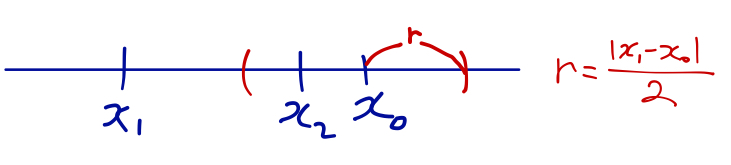
\includegraphics[height=2.5cm, width=12cm]{Oct26_image.jpeg}$$
    \item i.e. $\exists\;x_2\in B_r(x_0)$
    \item Then $|f(x_1)-f(x_2)| \ge \epsilon,$ but $|x_1-x_2|<2\delta$.
    \item So $f$ is not uniformly continuous.\\
    
    \item Consider $g(x)=\frac{1}{1+(x-x_0)^2}$.
    \item So $\forall\;x\in E,\; |g(x)|<1$, $g$ is continuous and as $x\to x_0,\; g(x)\to k,$ so $\sup\{g(x)\;|\;x\inE\}=1,$ but supremum is not attained.
    \item If $E$ is unbounded, $f(x)=x$ is continuous and unbounded.
    \item Consider $h(x)=\frac{x^2}{1+x^2},$ so $|h(x)|<1\;\;\forall\;x,\; \sup h=1$.
\end{itemize}

\end{document}